\documentclass[11pt,a4paper]{article}

% ── Packages ──────────────────────────────────────────────────────────────
\usepackage[utf8]{inputenc}
\usepackage[T1]{fontenc}
\usepackage{amsmath,amssymb,amsthm}
\usepackage{amscd}
\usepackage{booktabs}
\usepackage{graphicx}
\usepackage{array}
\usepackage{tikz}
\usetikzlibrary{arrows.meta,positioning,fit,backgrounds}
\usepackage{hyperref}
\usepackage[margin=1in]{geometry}
\usepackage{enumitem}
\usepackage{xcolor}
\definecolor{hlblue}{RGB}{0,80,160}
\hypersetup{colorlinks=true,linkcolor=hlblue,urlcolor=hlblue,citecolor=hlblue}

% ── Theorems ──────────────────────────────────────────────────────────────
\newtheorem{principle}{Principle}[section]
\newtheorem{theorem}{Theorem}[section]
\newtheorem{definition}[theorem]{Definition}
\newtheorem{proposition}[theorem]{Proposition}
\newtheorem{corollary}[theorem]{Corollary}
\theoremstyle{remark}
\newtheorem{remark}[theorem]{Remark}

% ── Shorthands ────────────────────────────────────────────────────────────
\newcommand{\Reg}{\ensuremath{\mathsf{M}}}          % number of registers
\newcommand{\Prec}{\ensuremath{P}}                  % precision
\newcommand{\Bits}{\ensuremath{b}}                  % bits per register
\newcommand{\Lat}{\ensuremath{\mathcal{B}}}         % the ambient EWM lattice
\newcommand{\Plane}{\ensuremath{\mathbb{B}}}        % one world's bit plane
\newcommand{\Tok}{\ensuremath{\mathcal{T}}}         % token space
\newcommand{\muw}{\ensuremath{\mu_{w}}}             % world measurement
\newcommand{\Img}{\ensuremath{\mathrm{Im}}}         % image / join-closure
\newcommand{\Lut}{\ensuremath{\mathcal{L}}}         % LUT
\newcommand{\iotaw}{\ensuremath{\iota_{w}}}         % world interpretation
\newcommand{\Bnd}{\ensuremath{\Phi}}                % bridge
\newcommand{\op}{\ensuremath{\oplus}}

% ── Title ─────────────────────────────────────────────────────────────────
\title{\textbf{The EWM Lattice and Its Worlds}\\[4pt]
\large HLLSets, Emerging Lattices, and Multi-World Representation\\[6pt]
\normalsize Companion note to \textit{Emerging World Models} (August 2026)}
\author{Alex Mylnikov \and Alexandr Mylnikov Jr. \and Deependra Kumar}
\date{\today}

\begin{document}
\maketitle

\begin{abstract}
This companion note elaborates the object at the center of the Emerging World
Models (EWM) framework: the \textbf{HLLSet lattice} and the \textbf{worlds} it
carries. The important word in EWM is \emph{emerging}. The lattice is never
built whole; it is grown as measurements arrive. An HLLSet is a compact
bit-vector ``sketch'' of a token collection, and the HLLSet algebra
(\emph{one universe}: every sketch is a node of one Boolean lattice; \emph{the
morphism is the contract}: a deterministic, immutable, content-addressed map
from tokens to nodes) is what makes the growth safe. Many users---many
\textbf{worlds}---can write into the same lattice simultaneously, and the
algebra makes it impossible for them to build anything wrong: the join is
monotone and convergent, so independent contributions coexist rather than
conflict. The hash function (its \emph{type} and its \emph{seed}) is a
parameter of the measurement, not part of the lattice, so different users hash
into different worlds that are \emph{virtually isolated even when they share
HLLSets}: a shared sketch is the same node on the representation plane, but
each world reads it through its own LUT. This built-in isolation is a free
consequence of the algebra, not a bolt-on policy; we call it the
\emph{emergence security} of HLLSet Algebra. We formalize worlds as
BSS-thresholded node sets with interpretations, prove the closure and isolation
properties, describe the internal sub-pipeline by which two worlds communicate
(materialize in world~1, transcribe, ingest in world~2), and close by
identifying the bridge with the Grothendieck-topology target of the main paper.
The lattice's size---$2^{32\mathrm{K}}$ nodes at the default configuration---is
treated in a single paragraph as the variety a compact presentation affords.
\end{abstract}

% ==========================================================================
\section{Introduction}
% ==========================================================================

The main EWM paper~\cite{ewm2026} establishes four foundation principles and
grounds them in HLLSet Algebra~\cite{astesj2026}. Its Section~5 (``HLLSet
Algebra: Concrete Instantiation'') treats the HLLSet bitmask as a holographic
plate of $32{,}768$ patches, and its Section~7 (``Toward Grothendieck
Topology'') anticipates geometric morphisms as universal bridges. The present
note is the missing middle: it takes the object that the
\texttt{ewm-state-machine} project actually materializes---the \textbf{HLLSet
lattice}, and the \textbf{worlds} that coexist on it---and develops the
structural consequences that the framework has been using informally.

The word that carries most of the weight in \emph{Emerging World Models} is
\textbf{emerging}. We never build a whole dense HLLSet lattice; there is no
reason to, and at the default configuration there could be no hope of it. The
lattice is built \emph{as we go}, node by node, as measurements arrive. What
makes this safe at scale is HLLSet Algebra, which gives three things:

\begin{enumerate}[leftmargin=*,nosep]
  \item \textbf{One universe.} Every HLLSet is a node of one Boolean lattice
    (order $\subseteq$, join $\cup$, meet $\cap$, ring $\Delta$). Nothing is
    created that was not already a node; a computation \emph{discovers} a node
    by naming a lattice expression. Building the lattice is discovering nodes,
    never restructuring it.
  \item \textbf{The morphism is the contract.} The token$\to$node connection is
    a chosen measurement morphism; only its IICA properties---Idempotence,
    Immutability, Content Addressability---are required, and any IICA algorithm
    is interchangeable. The bit vector is anonymous: it does not remember which
    token or which scheme set it.
  \item \textbf{Monotone, convergent accumulation.} The join is union, and union
    is idempotent, commutative, and associative. Independent contributions
    therefore accumulate without coordination, without consensus, and without
    conflict.
\end{enumerate}

The consequence is the theme of this note: \textbf{many users---many
worlds---can write into the same lattice simultaneously, and the algebra makes
it impossible for them to build anything wrong.} A node that one user adds is a
node the lattice now has; another user adding overlapping nodes cannot corrupt
it, because union is monotone and content-addressed. There is no lock, no
registry, and no validation pass to get wrong.

The hash function (its \emph{type} and its \emph{seed}) enters as a parameter of
the measurement, not as part of the lattice. That single choice partitions the
users into \textbf{virtually isolated worlds}: two users who hash differently
generally place the same token at different nodes, and they read any shared node
through their own LUTs. Even when they \emph{share} HLLSets, each world's
interpretation of those sketches is its own. This is a built-in isolation that
HLLSet Algebra gives us \emph{for free}---the \emph{emergence security} of the
representation. We make it precise in Sections~\ref{sec:worlds}--\ref{sec:bridge}.

% ==========================================================================
\section{HLLSets and the Emerging Lattice}
\label{sec:lattice}
% ==========================================================================

\subsection{What an HLLSet is}

An \textbf{HLLSet} is a compact sketch of a token collection. Instead of storing
the tokens, it stores a fixed-length bit vector whose set bits are the
\emph{measurement sites} the tokens hashed into. It is the object the
\texttt{ewm-state-machine} project manipulates: a token stream goes in, one
sketch comes out, and the sketch is what all later computation reads.

The geometry of the sketch is \emph{soldered}:
\begin{itemize}[leftmargin=*,nosep]
  \item precision $\Prec$ fixes the \textbf{register count} $\Reg = 2^{\Prec}$;
  \item each register occupies $\Bits$ bits of the flattened vector;
  \item a token $t$ is hashed once and decomposed into a \emph{register index}
    and a \emph{trailing-zero state}, which together name a single
    \textbf{bit address} in the vector.
\end{itemize}

The decomposition is the insertion rule
\begin{equation}
  \label{eq:position}
  \mathrm{reg}(t) = h(t) \bmod \Reg,
  \qquad
  \mathrm{tz}(t) = \mathrm{clamp}\bigl(\mathrm{trailing\_zeros}(h(t) \gg \Prec),\,
  0,\, \Bits-1\bigr),
\end{equation}
and the address is the flat pair
\begin{equation}
  \label{eq:bit}
  \mathrm{bit}(t) \;=\; \mathrm{reg}(t)\cdot \Bits + \mathrm{tz}(t)
  \;\in\; \{0,1,\dots,\Reg\cdot\Bits-1\}.
\end{equation}

\begin{definition}[HLLSet]
\label{def:hllset}
Fix a token space $\Tok$. The \textbf{bit plane} is
$\Plane = \{0,\dots,\Reg\cdot\Bits-1\}$, and an \textbf{HLLSet} is a subset
$H \subseteq \Plane$, represented by its indicator vector---a flattened bit
vector of length
\begin{equation}
  \label{eq:vectorlength}
  \Reg\cdot\Bits \;=\; 2^{\Prec}\cdot\Bits.
\end{equation}
The sketch of a token collection $A \subseteq \Tok$ is
\begin{equation}
  \label{eq:sketch}
  H(A) \;=\; \bigcup_{t\in A}\bigl\{\mathrm{bit}(t)\bigr\},
\end{equation}
so a token collection is represented by the set of sites it marks, not by the
tokens themselves. With the defaults $\Prec=10$ and $\Bits=32$ the vector is
$32{,}768$ bits long---a $32$K-bit presentation.
\end{definition}

\subsection{The HLLSet lattice}

The one fact that turns sketches into a representation is that subsets of a
common plane are automatically a lattice: inclusion orders them, union joins
them, intersection meets them.

\begin{definition}[The HLLSet lattice]
\label{def:lattice}
Let $\Plane = \{0,\dots,\Reg\cdot\Bits-1\}$ be the bit plane. The
\textbf{HLLSet lattice} (the EWM lattice) is the Boolean lattice
\begin{equation}
  \Lat \;=\; \bigl(\,2^{\Plane},\; \subseteq,\; \cup,\; \cap,\; \Delta\,\bigr),
\end{equation}
with order $\subseteq$ (bitwise subset), join $\cup$ (bitwise OR), meet $\cap$
(bitwise AND), and ring addition $\Delta$ (symmetric difference). An HLLSet is
a node of $\Lat$---one $32$K-bit presentation---and every computation in the
state machine---unions, R-links $A\cap B$, the DRN decomposition, ring
residuals, basis frames---names a node and \emph{discovers} it rather than
creating it.
\end{definition}

Three of the algebra's properties are what the rest of the note relies on, and
they are worth stating once, plainly:
\begin{enumerate}[leftmargin=*,nosep]
  \item \textbf{One universe.} Every HLLSet is a node of the same $\Lat$;
    nothing is created that was not already a node. A computation
    \emph{discovers} a node by naming a lattice expression, and two paths that
    name the same expression reach the same node.
  \item \textbf{The morphism is the contract (IICA).} The token$\to$node
    connection is a chosen measurement morphism
    $\mu:\{\text{token collections}\}\to\{HLLSets\}$; the only requirement is
    that $\mu$ be Idempotent, Immutable, and Content-Addressed. The bit vector
    forgets provenance by design, and any IICA algorithm is interchangeable.
  \item \textbf{Monotone, convergent accumulation.} The join is $\cup$, which is
    idempotent, commutative, and associative. Independent contributions
    therefore accumulate without coordination, consensus, or conflict.
\end{enumerate}

\begin{remark}
The bit-plane lattice is exactly the ``one universe'' of the project's
\texttt{BOOLRING.md}: every HLLSet is a node of the same Boolean lattice, and
every morphism result already exists in it. Definition~\ref{def:lattice} is the
paper-level statement of that fact.
\end{remark}

\subsection{Emerging: the lattice is grown, never built whole}
\label{sec:emerging}

We never materialize a dense HLLSet lattice, and there is no reason to try. At
the default configuration it has $2^{32\mathrm{K}}$ nodes, of which only a
vanishing fraction will ever be needed. The lattice is \textbf{emerging}: it is
grown node by node as measurements arrive.

Concretely, a site subscribes to the tokens it cares about, hashes each one
through $\mu$, and unions the resulting site into the sketches it holds. The
set of nodes in existence is the set of expressions the participants have
actually named---the committed sketches, their unions and intersections, their
DRN components, their ring residuals. Nothing else exists, and nothing else
needs to. This is what makes the representation scale: the cost is proportional
to the measurements taken, not to the size of the plane they could occupy.

The monotonicity of $\cup$ is what makes the growth safe, and it is why
\emph{many users can write into the same lattice at once}. Suppose users
$u_1,\dots,u_m$ independently add their sketches. Whatever order the additions
arrive in, and however they interleave, the accumulated node is the union of
their contributions; union is associative, commutative, and idempotent, so the
final node is independent of interleaving and re-addition. A user cannot
overwrite another's node, cannot leave the lattice in an inconsistent state,
and cannot even tell (from the lattice alone) that anyone else is writing. The
algebra makes it impossible to build anything wrong.

\begin{principle}[Emergence safety]
\label{prin:emergence}
A shared HLLSet lattice can be written concurrently by any number of
independent participants. Every contribution is a monotone join, and joins
commute, associate, and absorb repetition; hence the accumulated state is
well-defined and order-independent, and no participant can corrupt another's
contribution. There is no lock, no registry, and no consensus protocol to
implement.
\end{principle}

\begin{remark}[Variety from a compact presentation]
It costs one paragraph to say how much room this gives us. The flattened vector
has $\Reg\cdot\Bits = 32\mathrm{K}$ bit positions, so the lattice has
$2^{\,\Reg\cdot\Bits} = 2^{32\mathrm{K}} = 2^{32768}$ nodes at the defaults
($\Prec=10$, $\Bits=32$); that is a $9{,}865$-digit number, about $2^{32502}$
times the count of atoms in the observable universe. The point is not the
number itself---we will never visit more than a sliver of it---but that a
presentation of $32\mathrm{K}$ bits (4 KB, when packed) can name so vast a
variety of distinct states. That is the room in which the worlds of the next
section emerge.
\end{remark}

% ==========================================================================
\section{The Hash Function as an Index of Worlds}
\label{sec:worlds}
% ==========================================================================

\subsection{The hash configuration}

The insertion rule~\eqref{eq:position} depends on a hash function. In the
project it is MurmurHash3 x64-128 (lower 64 bits)~\cite{murmur3}, and the
realization exposes two independent choices:
\begin{itemize}[leftmargin=*,nosep]
  \item the \textbf{hash type} (which algorithm);
  \item the \textbf{seed} $s$, already present in the interface as
    \texttt{murmur3\_hash\_seeded(data, seed)}.
\end{itemize}
We call the pair $(h,s)$ a \textbf{hash configuration}---it is the $h$-part of a
world, as formalized next. A bootstrap scheme
(e.g.\ $n$-gram windows versus $n$-seed catalogs, with the channel seeds
$\mathrm{seed}(n,\dim)=(\dim-1)\cdot 3+(n-1)$) is a further, encoding-level
choice; it enters the same framework as a discrete family of seeds, and we
return to it in Section~\ref{sec:worlds-schemes}.

\begin{definition}[World]
\label{def:world}
A \textbf{world} is a triple $w=(h,s,\tau)$:
\begin{itemize}[leftmargin=*,nosep]
  \item a hash configuration $(h,s)$ (hash type and seed), which induces the
    \textbf{measurement morphism}
    \begin{equation}
      \muw : 2^{\Tok} \longrightarrow 2^{\Plane},
      \qquad
      \muw(A) \;=\; \bigcup_{t\in A}\bigl\{\mathrm{bit}_{h,s}(t)\bigr\},
    \end{equation}
    with $\mathrm{bit}_{h,s}$ as in~\eqref{eq:bit}; the \textbf{world image}
    $\Img(w)=\muw(2^{\Tok})$ is the set of atoms it can produce, and the
    \textbf{world lattice}
    \begin{equation}
      \Lat_w \;=\; \text{join-closure of } \Img(w) \;\subseteq\; \Lat
    \end{equation}
    is its set of \emph{reachable nodes} (every finite union of world atoms);
  \item a BSS threshold $\tau$. Writing
    \begin{equation}
      \mathsf{BSS}_w(X) \;=\; \frac{|X\cap B_w|}{|B_w|}
    \end{equation}
    for the BSS of a node $X$ against the world's basis $B_w$ (the ring over
    that world's HLLSets), the \textbf{thresholded node set}
    \begin{equation}
      \label{eq:thresholded}
      \mathcal{N}_\tau(w) \;=\;
      \bigl\{\,X\in\Lat_w \;:\; \mathsf{BSS}_w(X)\ge\tau\,\bigr\}
    \end{equation}
    is the collection of nodes that belong to the world, together with the
    relations between them that pass $\tau$;
  \item an \textbf{interpretation}
    \begin{equation}
      \label{eq:interpretation}
      \iotaw : 2^{\Plane} \longrightarrow 2^{\Tok},
      \qquad
      \iotaw(X) \;=\; \bigcup_{b\in X}\Lut_w[b],
    \end{equation}
    the materialization map that reads a node's active bits back as the tokens
    they stand for under $(h,s)$, through the reverse index $\Lut_w$ of that
    hash configuration (one fiber per bit address).
\end{itemize}
The thresholded node set is the world's extent; the interpretation is the
world's reading of it. Two worlds are \textbf{the same world} when both their
thresholded node sets and their interpretations agree on the nodes they share;
they are \textbf{distinct worlds} otherwise.
\end{definition}

In the state machine, a world is therefore what is left after the BSS threshold
is applied---the surviving nodes and relations---together with the LUT that
gives those nodes their meaning. The threshold is what makes the collection a
\emph{world} rather than a bare sublattice; the interpretation is what makes it
this world rather than another.

\begin{proposition}[Same hash type, different seeds]
\label{prop:isomorphism}
Let $w=(h,s)$ and $w'=(h,s')$ use the same hash type with different seeds. On
the common token domain, the two measurements are related by a bijection of
atoms $\phi:\Img(w)\to\Img(w')$, and $\phi$ extends uniquely to a lattice
isomorphism $\widehat{\phi}:\Lat_w\to\Lat_{w'}$ that commutes with
$\cup,\cap,\Delta$.
\end{proposition}

\begin{proof}
Both worlds realize the same abstract map
$\text{token}\to(\text{register},\text{tz})\to\text{bit}$; only the two hash
values differ. On each token $t$, set
$\phi(\mathrm{bit}_{h,s}(t))=\mathrm{bit}_{h,s'}(t)$. Distinct tokens can give
the same atom (collisions), so $\phi$ is well defined as a map of atoms exactly
when collisions agree; where they do, the induced map on the generated Boolean
algebras is the unique lattice homomorphism extending $\phi$, and it is a
bijection because both worlds generate free Boolean algebras on the same token
domain modulo the same collided partition. Boolean operations on a bit plane are
coordinatewise, so $\cup,\cap,\Delta$ are carried to $\cup,\cap,\Delta$.
\end{proof}

Changing the hash \emph{type}, not only the seed, likewise changes the realized
atom map, not the algebra. This is the precise sense in which EWM is
hash-agnostic.

\begin{theorem}[Closure of a world's representation under computation]
\label{thm:closure}
Let $W_1,\dots,W_k\in\Lat_w$. Let
\begin{equation*}
  E \;=\; E\bigl(W_1,\dots,W_k\bigr)
\end{equation*}
be any expression built from the operations $\cup,\cap,\setminus,\Delta$ and the
constants $\varnothing,\Plane$. Then $E\in\Lat_w$. In particular, the DRN
components $D=A\setminus B$, $R=A\cap B$, $N=B\setminus A$, the ring residual,
and every basis-frame projection of a world's HLLSets remain in that world.
\end{theorem}

\begin{proof}
$\Lat_w$ is by construction the Boolean subalgebra of $\Lat$ generated by the
atoms $\Img(w)$: it is closed under finite union and complement, hence under the
derived operations $\cap,\setminus,\Delta$ and contains
$\varnothing,\Plane$. Each $W_i$ is a finite union of atoms of $\Img(w)$; any
expression $E$ is therefore a finite Boolean combination of those atoms, which
lies in the generated subalgebra. Induction on the expression $E$ gives the
claim.
\end{proof}

The theorem is a statement about the \emph{representation} plane. The
interpretation layer is not closed in this way---$\iotaw$ need not commute with
$\cup,\cap$ beyond the fiber union it is defined by---and that asymmetry is
exactly what makes worlds separate: computing inside a world stays in its
representation, while \emph{reading} it requires that world's LUT. Shared
representation, separate interpretation.

\subsection{Interpretation and the separation of worlds}
\label{sec:twolevels}

The representation plane is uniform across worlds: there is one ambient lattice
$\Lat$, and every world's nodes are nodes of it. A world cannot therefore be
separated from another by \emph{which nodes exist}---they all live in the same
$2^{32\mathrm{K}}$-node lattice. What distinguishes worlds is how the nodes are
\emph{read}. The formal objects of Definition~\ref{def:world} split accordingly:
the thresholded node set $\mathcal{N}_\tau(w)$ is set-theoretic, and the
interpretation $\iotaw$ is the reading applied to it.

\begin{proposition}[Representation-level sharing, interpretation-level separation]
\label{prop:twolevels}
Two worlds may share the very same HLLSet node $X$ yet be distinct worlds.
They are distinct exactly when the interpretations differ on a shared node,
\begin{equation}
  w\neq w' \quad\Longleftrightarrow\quad
  \exists\,X\in\mathcal{N}_\tau(w)\cap\mathcal{N}_{\tau'}(w'):
  \;\iotaw(X)\neq\iota_{w'}(X),
\end{equation}
and their interpretations may still overlap,
$\iotaw(X)\cap\iota_{w'}(X)\neq\varnothing$, when the two token sets share
tokens while differing elsewhere.
\end{proposition}

\begin{proof}
Let $X$ be a node reachable under both configurations (a shared HLLSet, e.g.\ a
constant node or a node of common structure). Definition~\ref{def:world}
assigns to $X$ the token set $\iotaw(X)$ under $w$ and $\iota_{w'}(X)$ under
$w'$. If the two assignments differ, $X$ is the same bit vector in both worlds
but two different readings; this is separation with shared representation. The
converse is the definition of distinctness. Overlap of the two readings is
possible because the fibers $\Lut_w[b]$ and $\Lut_{w'}[b]$ are different sets of
tokens that may intersect; nothing forces disjointness.
\end{proof}

\begin{proposition}[Hash configurations give distinct worlds]
\label{prop:distinct}
Suppose the token domain is rich enough that two different hash configurations
$w=(h,s)$ and $w'=(h',s')$ separate on some token, i.e.\
$\mathrm{bit}_{h,s}(t)\neq\mathrm{bit}_{h',s'}(t)$ for some $t\in\Tok$. Then
$w$ and $w'$ are distinct worlds in the sense of Definition~\ref{def:world}.
\end{proposition}

\begin{proof}
The two configurations place $t$ at different bit addresses. Hence the fiber
containing $t$ under $\Lut_w$ is indexed by an address different from the one
under $\Lut_{w'}$; materializing a node that contains the address of $t$ under
$w$ returns $t$ (among others), while the corresponding reading under $w'$
reads a different fiber. So the interpretations differ on that node.
\end{proof}

The decisive point is that the bit vector itself is semantically inert: nothing
in the HLLSet remembers that it was produced under $h$ rather than $h'$. All
meaning lives in the LUT, and the LUT is a different object for every hash
configuration. Worlds are separated by their LUTs, not by their bit vectors.

\begin{corollary}[No cross-talk, restated]
\label{cor:notalk}
Inferring world $w'$ from world $w$ cannot be done by the lattice operations
alone: by Proposition~\ref{prop:twolevels} a node read under $w'$ differs from
the same node read under $w$ exactly at the interpretation step, which the
lattice does not perform. The two worlds meet only in the shared representation,
where they are indistinguishable until materialized; to go from one to the
other one must materialize and re-ingest---the bridge of
Section~\ref{sec:bridge}.
\end{corollary}

This is the technical content of the phrase ``all these worlds stay fully
isolated in this EWM lattice''. Isolation is not enforced by a lock, a namespace,
or a validation pass; it is a consequence of the interpretation layer being a
\emph{module over the representation}: every world has the same nodes, and each
world reads them through its own LUT.

\begin{principle}[Virtual isolation as built-in security]
\label{prin:virtual-isolation}
Two users who hash differently inhabit \textbf{virtually isolated worlds} on one
shared lattice. At the representation level they genuinely share nodes---the
sketch of a common token collection is the same bit vector for both---but at the
interpretation level $\iotaw$ recovers tokens through the LUT of $(h,s)$. A user
who does not hold the other's hash configuration and LUT cannot read the
content their node stands for, however much of the lattice they inspect. The
isolation is not a policy applied on top of the data; it is a property of the
algebra, and it is therefore obtained for free.
\end{principle}

\begin{remark}[What ``for free'' means here]
The representation is whole and shared: we do not partition, encrypt, or gate
the bit plane. \emph{Virtual} isolation means that the separation is carried by
the interpretation, so it costs one hash configuration and one LUT per world,
not a division of the lattice. It also means the separation is
\emph{structural rather than adversarial-tamper-proof}: it prevents
\emph{reading} another world's content and prevents \emph{confusing} one world's
nodes with another's, but it is not a substitute for cryptography where an
adversary can choose the encodings. Its value is that a representation built
for one purpose cannot silently leak into, or be corrupted by, a representation
built for another.
\end{remark}

\subsection{The lattice as a holographic presentation of many worlds}

Write $\Omega$ for the space of hash configurations $w=(h,s)$, and let
$\Lat_\Omega=\bigcup_{w\in\Omega}\Lat_w$ be the union of all reachable nodes
across the family. Because the ambient lattice is a single object, the
collection of worlds is not a collection of separate memories; it is a family of
\emph{readings} of one memory.

\begin{principle}[Holographic multi-worlds]
\label{prin:holographic}
Let $\Omega$ be any finite or countable family of hash configurations. Then:
\begin{enumerate}[leftmargin=*,nosep]
  \item \textbf{Common representation.} Every world $w\in\Omega$ is read
    through the same lattice $\Lat$; the representation is not duplicated per
    world. All worlds have access to the full $2^{32\mathrm{K}}$ nodes.
  \item \textbf{Separate interpretation.} What makes two worlds distinct is
    their interpretation map $\iotaw$ (Definition~\ref{def:world}),
    not their nodes: they may share a node exactly and still differ
    (Proposition~\ref{prop:twolevels}).
  \item \textbf{Joint closure of the representation.} Every expression over
    nodes drawn from a \emph{single} world stays in that world's subalgebra
    (Theorem~\ref{thm:closure}); the thresholded node set
    $\mathcal{N}_\tau(w)$ is the world's actual extent.
  \item \textbf{Global representability.} The whole of $\Lat_\Omega$ is a
    subset of one $2^{32\mathrm{K}}$-node lattice; the cost of hosting
    $|\Omega|$ worlds is a per-world LUT and threshold, not a multiplication of
    the representation.
\end{enumerate}
\end{principle}

The word \emph{holographic} is used in the same sense as in the main paper: the
lattice top plus its local coordinates reconstructs each world's state, and a
world is a \emph{view} of the whole. Formally, the structure over $\Omega$ is
not the disjoint union of the representations---those all coincide, being the
same $\Lat$---but the fibred set
\begin{equation}
  \mathcal{E}(\Omega) \;=\; \biguplus_{w\in\Omega}
  \bigl(\,\mathcal{N}_\tau(w),\; \iotaw\,\bigr)
\end{equation}
whose fibre at $w$ is that world's thresholded node set together with its
interpretation. The shared representation supplies the base geometry; the
fibre supplies the reading. Reading a world is choosing a fibre; reading all
worlds at once is reading the total space $\mathcal{E}(\Omega)$ through the one
common $\Lat$.

\begin{remark}[Why the worlds do not multiply the cost]
If the worlds had separate representations, the state-bit budget would be
$|\Omega|\cdot \Reg\cdot\Bits$. In the holographic arrangement the representation
budget stays $\Reg\cdot\Bits$ bits \emph{shared}; each world adds only its LUT
and its threshold. Since the cache stores a bounded working set (the ring, the
tip, the committed turns), the practical overhead is the per-world LUT, not the
lattice.
\end{remark}

\subsection{Adding bootstrap schemes to the family}
\label{sec:worlds-schemes}

The bootstrap scheme is a second, encoding-level parameter and fits the same
picture. An $n$-gram over a stream and an $n$-seed catalog over the same tokens
use different channel seeds,
\begin{equation}
  s(n,\dim) = (\dim-1)\cdot 3 + (n-1),
  \qquad s(1,\cdot)=0,
\end{equation}
and therefore are different worlds $(h,s(n,\dim),\tau)$ in the sense of
Definition~\ref{def:world}. The scheme lives on the \emph{LUT name}
(\texttt{ng:} versus \texttt{ns:}), which is the materialization coordinate of
the world; the HLLSet itself stays scheme-agnostic, exactly as the project's
\texttt{SEPARATION.md} insists. Thus the hash-configuration part of the world
family is
\begin{equation}
  \Omega \;=\; \bigl\{\,w=(h,s)\;:\; h\in\text{hash types},\;
  s\in\text{seeds}\cup\{s(n,\dim)\}_{n,\dim}\,\bigr\},
\end{equation}
a discrete parameter space whose points are the worlds (each with its own BSS
threshold and interpretation $\iotaw$). Precision and register width, by
contrast, are not points of $\Omega$; they size the lattice itself
(Section~\ref{sec:lattice}) and are fixed before the world family is
considered.

\subsection{Content addressing and the multi-hash extension}
\label{sec:multihash}

A world's nodes are immutable and content-addressed, so each carries a key. In
the realization, the default key is a SHA-1 digest of the HLLSet itself. One
SHA-1 key, however, has only $2^{160}$ possible values, while the lattice has
$2^{32\mathrm{K}} = 2^{32768}$ nodes. A single digest therefore cannot name the
lattice injectively, and as the number of stored HLLSets grows the key space
becomes a hard ceiling. The gap is not marginal.

\begin{theorem}[Single-hash capacity bound]
\label{thm:single-hash}
No function whose output is a single $b$-bit hash is injective from the HLLSet
lattice $\Lat$ to its keyspace when $b < 32\mathrm{K}$. In particular, for
$b$-bit SHA-1 ($b=160$) across $N$ stored HLLSets the addresses collide when
$N$ approaches $2^{\,b/2} = 2^{80}$, and no key assignment with one digest can
cover more than $2^{160}$ of the $2^{32768}$ nodes.
\end{theorem}

\begin{proof}
A function into $2^b$ values has image of size at most $2^b$, so it cannot be
injective on a domain of size $2^{32\mathrm{K}}$ once $b<32\mathrm{K}$; this is
the pigeonhole principle. For a random $b$-bit hash the birthday bound puts the
first collision at $N\sim 2^{b/2} = 2^{80}$; SHA-1 has $b=160$.
\end{proof}

\subsubsection{The concrete design: one HLLSet, three hashes, three LUTs}

The fix reuses the materializer's own pattern. There, the 1-gram and the 0-seed
are the \emph{same} hash-seed pair (the shared channel), and the other channels
are reached either by a different hash value (3-gram) or by a different seed
(3-seed). HLLSet identity is extended the same way, but on the HLLSet itself:
we take the HLLSet, hash it once for the default identifier and rehash the same
HLLSet under two further independent hashes.
\begin{equation}
  \label{eq:concrete}
  \kappa_3(H) \;=\; \bigl(\;
  \mathrm{SHA1}(H),\;
  \mathrm{H}_1(H, s_1),\;
  \mathrm{H}_2(H, s_2)
  \;\bigr),
\end{equation}
where $H$ is the HLLSet, $\mathrm{H}_1$ may be another 160-bit function or a
wider one such as Murmur-256, and $s_1\neq s_2$ are independent seeds. The three
digests are three names for the \emph{same} object; no token is involved, and
nothing about the sketch changes.

The vocabulary matters here. A LUT holds \emph{collections}: a token LUT holds
tokens (or token hashes), and an \texttt{hllsetLUT} holds HLLSets. The words
\emph{bucket} and \emph{register} are reserved for the internal structure of an
HLLSet and are not used for lookups. The correspondence is exact: every token
is kept in three token LUTs, and every HLLSet is kept in three
\texttt{hllsetLUT}s, under three different IDs, while the object is the same.
(This is the same move as the $n$-gram LUTs, where an $x$-gram is stored under
its own key and points at its first token; here the HLLSet is stored under three
keys and all three point at the same object.)

So the state machine keeps three \texttt{hllsetLUT}s, one per digest,
\begin{center}
\texttt{sha1-hllsetLUT}, \quad \texttt{hash1-hllsetLUT}, \quad
\texttt{hash2-hllsetLUT},
\end{center}
each mapping a digest to the collection of HLLSets registered under it,
\begin{equation}
  \label{eq:lut}
  \mathrm{L}_\text{sha1},\;\; \mathrm{L}_\text{h1},\;\; \mathrm{L}_\text{h2}
  \;:\; \text{digest} \;\longrightarrow\; \text{collection of HLLSets}.
\end{equation}
This mirrors the token side, where the same token appears in three LUTs, and the
$n$-gram side, where the same window is indexed under its own key. It is the
project's existing ``one LUT per channel'' bookkeeping, now applied per hash
rather than per token channel.

\paragraph{The second and third LUTs grow lazily.} A SHA-1 collision is close
to impossible at any realistic scale, so the extra LUTs are not populated
eagerly. An HLLSet $H$ is added to the second LUT \emph{only if its SHA-1
identifier collides} with an already-registered HLLSet, and to the third LUT
\emph{only if the second also collides}. In the overwhelmingly common case an
HLLSet lives in the first LUT alone; the second LUT is a de-collider consulted
only under a SHA-1 collision, and the third is a de-collider consulted only
under a collision in the second. The two extra LUTs therefore hold at most a
negligible fraction of the collection, and the memory cost of the whole scheme
is one key per HLLSet plus a rare second or third key.

\begin{definition}[Three-stage retrieval]
\label{def:retrieval}
Retrieval descends the LUTs only as far as it must:
\begin{enumerate}[leftmargin=*,nosep]
  \item \textbf{(stage 1, the common case)} look up the SHA-1 LUT at $a$. If the
    collection $\mathrm{L}_\text{sha1}(a)$ holds exactly one HLLSet, return
    it---no further hashes are computed;
  \item \textbf{(stage 2)} otherwise compute the second hash $b$ and look up the
    second LUT. If $\mathrm{L}_\text{h1}(b)$ holds exactly one HLLSet, return
    it;
  \item \textbf{(stage 3, essentially never)} otherwise compute the third hash
    $c$ and intersect the three collections,
    \begin{equation}
      \label{eq:intersection}
      \mathrm{L}_\text{sha1}(a) \;\cap\; \mathrm{L}_\text{h1}(b) \;\cap\;
      \mathrm{L}_\text{h2}(c) \;=\; \{H\}.
    \end{equation}
\end{enumerate}
Only the first hash is paid on the common path; the second is paid only when
the SHA-1 collection is contested, and the third only when the second is
contested too.
\end{definition}

\begin{proposition}[Retrieval is exact]
\label{prop:retrieval}
Let $H$ be stored under the lazy regime above, with digests $\mathrm{SHA1}(H)=a$
and, when computed, $\mathrm{H}_1(H)=b$, $\mathrm{H}_2(H)=c$. Then
\begin{enumerate}[leftmargin=*,nosep]
  \item \textbf{Completeness.} At every stage where $H$'s digest is looked up,
    $H$ is present: at stage~1 by registration; at stage~2 because
    $\mathrm{L}_\text{sha1}(a)$ was contested, which triggered $H$'s
    registration in the second LUT; at stage~3 because
    $\mathrm{L}_\text{h1}(b)$ was contested, which triggered its registration in
    the third. Hence retrieval always returns the target.
  \item \textbf{Uniqueness.} Any $H'\neq H$ returned by stage~3 lies in all
    three collections and therefore collides with $H$ on all three hashes,
    $\mathrm{SHA1}$, $\mathrm{H}_1$ and $\mathrm{H}_2$ simultaneously. For
    independent $b$-bit hashes this costs a factor $2^{-b}$ per extra
    coordinate---about $2^{-320}$ for the two extra---and requires the rare
    two-stage collision to have occurred at all.
\end{enumerate}
\end{proposition}

\begin{proof}
(1) Registration places $H$ in the second LUT exactly when a SHA-1 collision
makes stage~2 reachable, and in the third exactly when a second-LUT collision
makes stage~3 reachable; in each case the entry needed for that stage exists.
(2) Membership in the stage-3 intersection means
$\mathrm{SHA1}(H')=\mathrm{SHA1}(H)$ \emph{and}
$\mathrm{H}_1(H')=\mathrm{H}_1(H)$ \emph{and} $\mathrm{H}_2(H')=\mathrm{H}_2(H)$;
for independent $b$-bit hashes each coincidence costs a factor $2^{-b}$, giving
$2^{-160}$ per extra coordinate.
\end{proof}

\begin{remark}[Capacity, not adversarial strength]
The three coordinates together name up to $2^{480}$ values, well past the
$2^{80}$ single-key collision point, and the two extra LUTs cost only the two
additional digests per HLLSet. Two caveats are worth stating. The construction
assumes the three hashes are \emph{independent}; a single function re-seeded
still shares that function's structural weaknesses. And the purpose is
\emph{capacity and collision resolution}, not adversarial collision resistance:
SHA-1 is long broken for adversarial purposes, so a system that must resist a
computing adversary should use a modern hash family while keeping the same
three-coordinate retrieval.
\end{remark}

\subsubsection{The general extension}

If more than three coordinates are ever needed, the same construction extends
to an $m$-fold \emph{extendable key},
\begin{equation}
  \label{eq:multikey}
  \kappa_m(H) \;=\; \bigl(\mathrm{SHA1}(H),\, \mathrm{H}_1(H),\, \dots,\,
  \mathrm{H}_{m-1}(H)\bigr),
\end{equation}
with one LUT per coordinate, all indexed by the same $H$. The address
space is $2^{\,b\,m}$ instead of $2^b$, and the collision condition becomes
conjunctive.

\begin{proposition}[Multi-hash extension]
\label{prop:multihash}
Let $\kappa_m$ be an $m$-fold independent $b$-bit key as in~\eqref{eq:multikey}.
Then:
\begin{enumerate}[leftmargin=*,nosep]
  \item \textbf{Coverage.} $\kappa_m$ can address up to $2^{\,b\,m}$ distinct
    HLLSets. Full coverage of the lattice needs
    \begin{equation}
      m \;\ge\; \left\lceil \frac{32\mathrm{K}}{b} \right\rceil,
      \qquad\text{i.e.}\quad m \ge 205 \text{ for SHA-1 }(b=160),
    \end{equation}
    or $m\ge 128$ with SHA-256 ($b=256$).
  \item \textbf{Collision law.} $\kappa_m(H)=\kappa_m(H')$ with $H\neq H'$
    requires a simultaneous collision in all $m$ coordinates; its probability
    falls as $2^{-b}$ per additional coordinate, giving
    $\Pr[\text{collision}]\approx N^2/2^{\,b\,m+1}$ for $N$ stored HLLSets.
  \item \textbf{Practical choice.} Full-coverage integrity needs $m=205$, but
    the concrete three-coordinate design of \eqref{eq:concrete} is chosen for
    the actual scale: its intersection collides with probability below
    $2^{-300}$ for $N\le 2^{100}$, and the second coordinate alone already
    reduces the SHA-1 collection by $2^{-160}$.
  \item \textbf{Cost.} The key grows by $b$ bits per coordinate---20 bytes per
    SHA-1 coordinate---so the concrete $m=3$ key adds $40$ bytes, and even the
    full-coverage $m=205$ key is about $4.1$~KB, comparable to the HLLSet
    presentation it names.
\end{enumerate}
\end{proposition}

\begin{proof}
(1) The image of $\kappa_m$ lies in $(2^b)^m = 2^{bm}$ values, so injectivity
requires $bm\ge 32\mathrm{K}$; the ceiling follows. (2) A collision of the
tuples is the intersection of $m$ independent events, each of probability
$\approx N^2/2^{b+1}$; independence multiplies them, giving
$N^2/2^{bm+1}$. (3) Substituting $N=2^{100}$ and $m=3$ gives $2^{200}/2^{481}$;
$N=2^{80}$ and $m=2$ gives $2^{160}/2^{321}$. (4) Each coordinate contributes
$b$ bits, $b/8$ bytes.
\end{proof}

\begin{remark}[The multi-seed sketch as an injective address]
There is a second, representation-side route to the same end. Ingesting a
token collection under $m$ independent seeds produces $m$ HLLSets in $m$ bit
planes; the $m$-tuple of those bit vectors is itself the address, and the map
from a single-seed lattice to the multi-seed product,
\begin{equation}
  H \;\longmapsto\; (H_0,\dots,H_{m-1}), \qquad H_s = \text{sketch of } H
  \text{ under seed } s,
\end{equation}
is injective once the coordinates are independent---it is the same extension
seen from the representation rather than the key side. This is exactly the
multi-seed ingestion the materializer already runs (\texttt{SEEDS = [0,1,2]}
and the channel seeds $s(n,\dim)$): the $0$-seed is the shared default, and the
additional seeds are the extra coordinates, one catalog per seed.
\end{remark}

\begin{remark}[What is and is not assumed]
The extension assumes the $m$ coordinates are \emph{independent} hash
functions. Reusing one SHA-1 with a seed is a practical way to generate them,
but then the coordinates share SHA-1's structural weaknesses; the correct
reading is that the key is as strong as the weakest independent function used.
The point of Proposition~\ref{prop:multihash} is capacity, not adversarial
collision resistance: SHA-1 is long broken for adversarial purposes, and a
system that needs the latter should use a modern hash family while keeping the
same $m$-fold extension. The registry cost is the same either way.
\end{remark}

\begin{remark}[Where the LUTs keep it]
The \texttt{ewm-state-machine} already keeps touch-count \texttt{HllsetLut}s,
merged as a monotonic CRDT, one per token channel. The three-hash design adds
two more \texttt{hllsetLUT}s of the same kind, one per hash, and each LUT entry
is a \emph{collection} of HLLSets (a digest may be carried by several of them),
as LUTs hold collections by definition. Because the second and third LUTs are
grown lazily, they add essentially nothing to the steady-state cost---only the
rare collision populates them---while the per-entry touch counts are kept
exactly as in the single-LUT case. The extension is bookkeeping plus
collision-tolerant LUT collections, not a new data structure.
\end{remark}

% ==========================================================================
\section{Cross-World Communication}
\label{sec:bridge}
% ==========================================================================

\subsection{The internal sub-pipeline}

Two worlds cannot exchange lattice nodes directly---by
Corollary~\ref{cor:notalk} a world's nodes simply do not name the other world's
nodes. Communication must pass through the only interface the worlds share:
the \textbf{encodings}. The bridge from world $w_1$ to world $w_2$ is the
composition
\begin{equation}
  \label{eq:bridge}
  \Bnd_{w_1\to w_2}
  \;=\;
  \underbrace{\text{ingest}_{w_2}}_{\text{hash }h_2,s_2}
  \circ\;
  \underbrace{\text{transcribe}}_{\text{LUT fiber} \to \text{value}}
  \circ\;
  \underbrace{\text{materialize}_{w_1}}_{\text{bits} \to \text{LUT fiber}},
\end{equation}
where materialize is the LUT-first inverse read of $\mu_{w_1}$ (every candidate
of every active bit is kept), and transcribe is the protocol-level mapping that
turns a recovered encoding into a value world $w_2$ can hash. In diagram form:
\begin{equation}
  \begin{CD}
    \Lat_{w_1} @>{\text{materialize}}>> \Lut_{w_1}
    @>{\text{transcribe}}>> \text{encodings}\\
    @. @. @VV{\text{ingest, }h_2,s_2}V\\
    \Lat_{w_2} @<<{\text{measure}}< \Img(w_2) @<<{\mu_{w_2}}< \text{encodings}
  \end{CD}
\end{equation}
In the project's terms this is exactly the side-car loop run twice, with the
materialized output of the first pass used as the input stream of the second.
The two worlds share the same surrounding pipeline---input, LLM encoding,
materialization, restored input---and meet only at the encoding layer:
\begin{center}
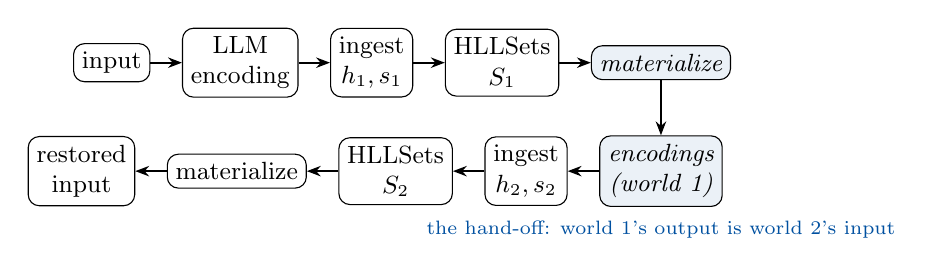
\begin{tikzpicture}[
    node distance=4mm,
    box/.style={draw, rounded corners, font=\small, inner sep=3pt, align=center},
    enc/.style={draw, rounded corners, font=\small\itshape, inner sep=3pt,
                fill=hlblue!8, align=center},
    ar/.style={-{Stealth[length=5pt]}, thick}]
  \node[box] (in) {input};
  \node[box, right=of in] (enc1) {LLM\\encoding};
  \node[box, right=of enc1] (h1) {ingest\\$h_1,s_1$};
  \node[box, right=of h1] (s1) {HLLSets\\$S_1$};
  \node[enc, right=of s1] (mat1) {materialize};
  \node[enc, below=7mm of mat1] (tok) {encodings\\(world 1)};
  \node[box, left=of tok] (h2) {ingest\\$h_2,s_2$};
  \node[box, left=of h2] (s2) {HLLSets\\$S_2$};
  \node[box, left=of s2] (mat2) {materialize};
  \node[box, left=of mat2] (out) {restored\\input};
  \draw[ar] (in) -- (enc1);
  \draw[ar] (enc1) -- (h1);
  \draw[ar] (h1) -- (s1);
  \draw[ar] (s1) -- (mat1);
  \draw[ar] (mat1) -- (tok);
  \draw[ar] (tok) -- (h2);
  \draw[ar] (h2) -- (s2);
  \draw[ar] (s2) -- (mat2);
  \draw[ar] (mat2) -- (out);
  \node[font=\scriptsize, text=hlblue, below=0.5mm of tok]
    {the hand-off: world 1's output is world 2's input};
\end{tikzpicture}
\end{center}

\begin{theorem}[Bridge laws]
\label{thm:bridge}
Let $\Bnd=\Bnd_{w_1\to w_2}$ be the bridge~\eqref{eq:bridge}, and assume
materialization is exact on the tokens that built the source nodes (the
standing guarantee of LUT-first materialization: every builder is returned).
Then:
\begin{enumerate}[leftmargin=*,nosep]
  \item \textbf{Determinism (IICA).} $\Bnd$ is deterministic and
    content-addressed: the same source state yields the same target node, and
    the target is named by its SHA-1 content key.
  \item \textbf{Idempotence on builders.} Ingesting the same bridge transcript
    again yields the same target node; hence $\Bnd^2=\Bnd$ on states whose
    materialization is exact.
  \item \textbf{Order preservation.} $\Bnd$ is monotone: $A\subseteq A'$ in
    $\Lat_{w_1}$ implies $\Bnd(A)\subseteq\Bnd(A')$ in $\Lat_{w_2}$.
  \item \textbf{Strict coarsening in general.} If materialization returns
    collateral candidates at collided bits, transcribing the larger transcript
    can only \emph{add} atoms to the target; $\Bnd$ is then a monotone
    inflation, not a bijection.
\end{enumerate}
\end{theorem}

\begin{proof}
(1) Materialize, transcribe, and ingest are each deterministic functions of
their inputs; composition preserves determinism and content addressability (the
IICA composition theorem of the main paper). (2) If materialization recovers
exactly the builders $B$ of the source node, the transcript is $B$; ingesting
$B$ under $(h_2,s_2)$ is $\mu_{w_2}(B)$, which is unchanged on a second pass
with the same transcript. (3) Materialization returns the builders of $A$; if
$A\subseteq A'$ then the builder set of $A$ is contained in that of $A'$ (up to
collisions), and $\mu_{w_2}$ is a union over the transcript, hence monotone.
(4) Collisions at materialization add candidates; ingest unions their atoms, so
the target can only grow.
\end{proof}

\subsection{What crosses the bridge, and what does not}

\begin{principle}[The bridge carries encodings, not content]
\label{prin:encodings}
The bridge $\Bnd_{w_1\to w_2}$ transmits the \textbf{encoded} form of the
state---token identifiers, codec tokens, n-gram windows, grid cells, or whatever
the world's front-end emits---and never the source content those encodings stand
for. The receiving world re-embeds the encoding under its own hash
configuration; it does not inherit the sender's semantics.
\end{principle}

This is not a defect but the architecture. The lattice is vocabulary-agnostic
and semantics-agnostic; it knows bits and their LUT fibers, not the meaning of
the tokens. Each side that participates in a bridge is responsible for its own
encoder and decoder. The bridge's guarantee is structural: \emph{the same
encodings, placed by the receiver's measurement, with the receiver's collisions
handled by its own LUT}. The fidelity of a bridge is therefore the fidelity of
the two encoders, not of the lattice; the lattice's contribution is that it
never loses a builder and never confuses two worlds.

\begin{remark}[Round-trips]
The composite $\Bnd_{w_2\to w_1}\circ\Bnd_{w_1\to w_2}$ is not the identity in
general: materializing extras from collisions, and re-encoding, can coarse-grain
the state. Exactness holds on the builders (Theorem~\ref{thm:bridge}(2)),
which is the sense in which the pipeline ``restores the input'': it restores the
\emph{encodings} exactly on everything that built the lattice state, and at most
adds hash-collision neighbours.
\end{remark}

\subsection{Communities of worlds}

The bridge composes, so a family of worlds connected by bridges forms a directed
graph whose vertices are hash configurations and whose edges are bridges. Two
consequences deserve to be stated because they are what the multi-world picture
buys:

\begin{itemize}[leftmargin=*,nosep]
  \item \textbf{Migration.} Information can be moved from a world with hash
    type $h_1$ to a world with hash type $h_2$ without re-architecting the
    lattice: only the two hash configurations and the transcription protocol
    must be agreed upon.
  \item \textbf{Adapters as bridges.} A new LLM, vision encoder, or decision
    model entering the system is a new vertex; its adapter is the transcription
    protocol on the incoming and outgoing edges. The \texttt{ewm-state-machine}
    project's repeated finding---\emph{the only model-specific code is a tiny
    adapter}---is the engineering face of Principle~\ref{prin:encodings}.
\end{itemize}

% ==========================================================================
\section{Correspondence with the Implementation}
% ==========================================================================

The definitions above are not idealized; each has a named counterpart in the
code. Table~\ref{tab:corr} collects them.

\begin{table}[t]
\centering
\small
\begin{tabular}{@{}p{0.36\textwidth}p{0.56\textwidth}@{}}
\toprule
This note & \texttt{ewm-state-machine} \\
\midrule
precision $\Prec$ & \texttt{hllset\_contracts::P = 10} \\
register count $\Reg=2^{\Prec}$ & \texttt{M = 1 << P = 1024} \\
bits per register $\Bits$ & \texttt{BITS\_PER\_REG = 32} \\
bit plane size $\Reg\cdot\Bits$ & \texttt{TOTAL\_BITS = 32768} \\
node of $\Lat$ & \texttt{hllset\_core::HLLSet} (a Roaring bitmap) \\
bit address & \texttt{hllset\_contracts::BitAddress} \\
$\mathrm{bit}=\mathrm{reg}\cdot\Bits+\mathrm{tz}$ & \texttt{BitAddress::from\_reg\_tz} \\
$\muw$, $w=(h,s)$ & \texttt{murmur3\_hash\_seeded} / \texttt{BitAddress::of\_token\_seeded} \\
$\mathrm{seed}(n,\dim)$ & \texttt{conv(n, dim)}; \texttt{SEEDS = [0,1,2]} \\
$\Img(w)$ & the content keys of the committed \texttt{HLLSet} nodes \\
$\mathsf{BSS}_w(X)=|X\cap B_w|/|B_w|$ & the BSS / similarity-coverage readouts \\
$\mathcal{N}_\tau(w)$ & the nodes surviving the world's BSS threshold \\
$\iotaw$ (interpretation) & LUT-first inverse read (\texttt{ewm-scene}, \texttt{LutIndex}) \\
content key of a node (default) & \texttt{h:\textless sha1\textgreater} (SHA-1 of the HLLSet) \\
additional hashes (two) & $\mathrm{H}_1(H,s_1)$, $\mathrm{H}_2(H,s_2)$ (eq.~\eqref{eq:concrete}) \\
three LUTs & \texttt{sha1-hllsetLUT}, \texttt{hash1-hllsetLUT}, \texttt{hash2-hllsetLUT} (digest $\to$ collection) \\
retrieval & SHA-1 LUT singleton, else the three-way intersection (Def.~\ref{def:retrieval}) \\
extendable key $\kappa_m$ & an $m$-tuple of independent digests (Proposition~\ref{prop:multihash}) \\
LUT type & \texttt{hllset\_morphisms::HllsetLut} ($(\textit{name},\textit{key})\to$ TH, CRDT) \\
materialize$_{w}$ & the interpretation applied to a node \\
ingest$_{w}$ & \texttt{hllset\_morphisms::Ingest} (+ \texttt{ns:G1..G3} LUTs) \\
$\Bnd_{w_1\to w_2}$ & the two-pass side-car loop (notebooks 02--21) \\
$\mathcal{E}(\Omega)$ & the \texttt{ewm-git} commit DAG over one shared store \\
\bottomrule
\end{tabular}
\caption{Correspondence between the lattice/world formalism and the artifacts
that realize it.}
\label{tab:corr}
\end{table}

Two implementation facts are worth calling out.

\paragraph{The world is a configuration, not a copy.}
Nothing in \texttt{hllset-core} or \texttt{hllset-contracts} knows about worlds.
The seed is a parameter of \texttt{BitAddress::of\_token\_seeded} and
\texttt{Ingest}; the hash type is a parameter of the hashing module. Reusing one
lattice across worlds is therefore already the default behaviour: there is no
``world'' type because there is nothing to switch---only a hash configuration to
vary, and a threshold to set.

\paragraph{Gates are single-world interpretations.}
The project's gates ($G_u$, and the G1-scoped \texttt{bss\_g1}) project a state
onto one dimension or one world's codebook. In the present language a gate is a
restriction of a world's interpretation $\iotaw$, not of the representation:
the one-sided gate (frames do not leak across a gate) is the operational shadow
of Corollary~\ref{cor:notalk}.

% ==========================================================================
\section{Relation to the Grothendieck-Topology Target}
% ==========================================================================

Section~7 of the main paper proposes Grothendieck topology as the target
formalism, with geometric morphisms as universal bridges. The construction of
this note supplies that target with its concrete objects:
\begin{itemize}[leftmargin=*,nosep]
  \item the \textbf{base site} is the discrete parameter space $\Omega$ of hash
    configurations;
  \item a \textbf{world} $w\in\Omega$ is a point of the base, and its stalk is
    the pair $(\mathcal{N}_\tau(w),\iotaw)$---the thresholded node set together
    with the interpretation, i.e.\ its fibre of $\mathcal{E}(\Omega)$;
  \item a \textbf{bridge} $\Bnd_{w_1\to w_2}$ is a morphism of sites: its
    ``direct image'' is the re-encoding $\text{ingest}_{w_2}$ and its ``inverse
    image'' is $\text{materialize}_{w_1}$, the pair being adjoint in the order
    of Theorem~\ref{thm:bridge}(3);
  \item the \textbf{pullback consistency} that a geometric morphism requires is
    the global-fiber invariant of the project's \texttt{SEPARATION.md}: within
    one world's LUT, one bit address points to the same fiber, so a
    materialization read is well defined. Across worlds the fiber is
    reinterpreted---that is exactly what makes the worlds distinct---and the
    bridge is the morphism that transports it.
\end{itemize}
What is still missing---and what we do not claim here---is the covering
structure (the analogue of the bootstrap covering families in the main paper)
and a genuine sheaf condition on $\Omega$. The bridge is a geometric morphism in
the order-theoretic sense; making it a morphism of sheaf toposes is future
work. Meanwhile the finite, fully explicit lattice of
Sections~\ref{sec:lattice}--\ref{sec:bridge} is the ``pre-sheaf'' stage of that
programme, exactly as the main paper describes its own status.

% ==========================================================================
\section{Summary}
% ==========================================================================

\begin{enumerate}[leftmargin=*,nosep]
  \item An \textbf{HLLSet} is a compact sketch of a token collection: a
    $32$K-bit vector at the defaults, marking the measurement sites the tokens
    hashed into. The \textbf{HLLSet lattice} $\Lat = 2^{\Plane}$ is the Boolean
    lattice of all such sketches (order $\subseteq$, join $\cup$, meet $\cap$,
    ring $\Delta$); every HLLSet is a node of it.
  \item The word \textbf{emerging} is literal: the lattice is \emph{grown}, never
    built whole. Participants name the node expressions they need (sketches,
    unions, intersections, DRN, ring residuals) and nothing else exists. The
    cost is proportional to the measurements taken, not to the
    $2^{32\mathrm{K}}$-node plane they could occupy.
  \item Because the join is union---idempotent, commutative, associative---%
    many users can write into the same lattice at once, and the algebra makes
    it \textbf{impossible to build anything wrong} (Principle~\ref{prin:emergence}).
    No lock, no registry, no consensus protocol.
  \item The \textbf{hash function (type and seed)} is a parameter of the
    measurement, so the same lattice carries a family of \textbf{worlds}
    $\Omega\ni w=(h,s)$. A world is its \emph{thresholded node set}
    $\mathcal{N}_\tau(w)$ together with its \emph{interpretation} $\iotaw$.
  \item Users who hash differently are \textbf{virtually isolated}: they may
    share the very same HLLSet and still read it differently, because each world
    recovers tokens through its own LUT (Principle~\ref{prin:virtual-isolation}).
    Separation lives at the interpretation level, not on the representation
    plane; it is a property of the algebra, obtained for free.
  \item Worlds communicate only through the \textbf{bridge}
    $\Bnd_{w_1\to w_2}=\text{ingest}_{w_2}\circ\text{transcribe}\circ{}\allowbreak
    \text{materialize}_{w_1}$, which is deterministic, idempotent on builders,
    and monotone, and which carries \textbf{encodings, not content}
    (Principle~\ref{prin:encodings}). The structure over $\Omega$ is the
    \textbf{holographic presentation} of the world family: one shared
    representation with per-world interpretation fibres, and the bridge is the
    concrete realization of the main paper's geometric-morphism target.
  \item A single SHA-1 key cannot name the lattice ($2^{160}$ against
    $2^{32768}$). The materializer's multi-hashing move fixes it at the HLLSet
    level: hash the same HLLSet under SHA-1 plus \textbf{two more hashes}
    (another $160$-bit function, or Murmur-256, under two seeds), one
    \texttt{hllsetLUT} per hash. The second and third LUTs are grown
    \textbf{lazily}, only on a collision at the preceding level, so a SHA-1
    lookup almost always settles retrieval on its own; escalation intersects
    the collections (Definition~\ref{def:retrieval},
    Proposition~\ref{prop:retrieval}). The coordinates name up to $2^{480}$
    values; the same construction extends to $m=205$ for full coverage
    (eq.~\eqref{eq:concrete}, Theorem~\ref{thm:single-hash},
    Proposition~\ref{prop:multihash}).
\end{enumerate}

% ==========================================================================
\section*{Acknowledgment}
% ==========================================================================
This article was written in collaboration between the authors---Alex Mylnikov
and Deependra Kumar---and an AI assistant (an instance of the DeepSeek model
working within the \texttt{ewm-jepa} workspace). The human authors developed the
EWM framework, the HLLSet algebra, and the \texttt{ewm-state-machine}
realization, and directed the line of argument; the AI assistant helped to
draft and structure the text, work through the formal statements and proofs,
and verify the correspondence with the implementation. The conceptual content
is the authors' own.

\begin{thebibliography}{9}
\bibitem{ewm2026} Alex Mylnikov, Deependra Kumar, \textit{Emerging World Models: A Structural
Framework for Self-Organizing World Representations}, consolidation document,
August 2026. (Main paper; companion to this note.)
\bibitem{astesj2026} \textit{HLLSet Algebra: A Content-Addressed Set Algebra for
Emergent Ontology}, ASTES Journal, 2026.
\bibitem{murmur3} A.~Appleby, \textit{MurmurHash3}, 2011. x64-128 variant; the
project uses the lower 64 bits with a configurable seed.
\bibitem{ashby1952} W.~R.~Ashby, \textit{Design for a Brain}, Chapman \& Hall,
1952; and \textit{An Introduction to Cybernetics}, 1956.
\bibitem{grothendieck1972} A.~Grothendieck et al., \textit{Th\'eorie des topos
et cohomologie \'etale de sch\'emas}, SGA~4, Lecture Notes in Mathematics~269,
Springer, 1972.
\bibitem{flajolet2007} P.~Flajolet, \'E.~Fusy, O.~Gandouet, and F.~Meunier,
\textit{HyperLogLog: the analysis of a near-optimal cardinality estimation
algorithm}, AofA, 2007.
\end{thebibliography}

\end{document}
